\documentclass{tktltiki}
\usepackage{ae,aecompl}
\usepackage{url}
\usepackage{amsfonts}
\usepackage{color}
\usepackage{graphicx}

% rubber: module pdflatex
% rubber: pdflatex.options -Ppdf -t a4

\begin{document}

\title{Salasanoista ei päästä eroon.\\ --- Mutta äheltämisestä päästään!}
\author{Petrus Repo}
\date{\today}
\level{Sosiaalisen median tekniikat -seminaari}
\maketitle


\onehalfspacing

\level{Seminaarityö}
\faculty{Matemaattis-luonnontieteellinen}
\department{Tietojenkäsittelytieteen laitos}
\subject{Tietojenkäsittelytiede}
\numberofpagesinformation{\numberofpages\ sivua}

\keywords{}

\begin{abstract}

\end{abstract}

\setcounter{tocdepth}{3}
\mytableofcontents


\section{Johdanto}

Jesjes.

\section{Autentikoituminen ja web}

Autentikoituminen on identiteetin määrittämistä. 

Jos \emph{s} on väite, autentikointi vastaa kysymykseen ''Kuka sanoi \emph{s}?''.
Jos \emph{o} on väitteen kohde, auktorisointi (\emph{authorization}) vastaa kysymykseen ''Kenellä on pääsy kohteeseen \emph{o}?'' \cite{lampson_distributed_1992}.


Haaste--vastine-autentikoinniksi (\emph{challenge-response authentication}) kutsutaan autentikointitapaa, jossa toinen osapuoli esittää kysymyksen (haasteen), johon toisen osapuolen on tarjottava kelvollinen vastaus (vastine) \cite{NIST_SP800-63}. 

Haaste voi olla satunnaisluku, jonka haastaja lähettää vastaajalle ja johon vastaaja yhdistää jonkin ennalta jaetun salaisuuden. Yhdistäminen voidaan tehdä esimerkiksi laskemalla tiiviste haasteesta ja salaisuudesta, joka lähetetään takaisin haastajalle. Koska haastaja tuntee jaetun salaisuuden, haastaja pystyy laskemaan oman versionsa tiivisteestä. Haaste voidaan hyväksyä, jos haastajan laskema ja vastaanottama tiiviste ovat identtiset \cite{NIST_SP800-63}.

Autentikoituminen käyttäjätunnuksella ja salasanalla on yksi haaste--vastine-autentikoinnin sovellus. 
Muita yleisiä haaste--vastine-autentikoinnin sovelluksia ovat esimerkiksi spämmiesto CAPTCHA-tunnistuksella.

Tämän paperin yhteydessä tiedonsiirtokanava oletetaan turvalliseksi, eikä yhteyden salakuuntelua käsitellä riskinä.


\subsection{Kaksiosainen autentikointi}

Kaksiosaisessa autentikoinnissa (\emph{two-factor authentication}) käyttäjälle esitetään kaksi haastetta. Ensimmäinen haaste edellyttää vastineeksi jotain, jonka käyttäjä \emph{tietää} (salasana). Toisen haasteen vastineeksi edellytetään jotain, jota käyttäjällä \emph{on} (esimerkiksi puhelinnumero) \cite{NIST_SP800-63, google_2step_2010}. Jälkimmäinen tekijä voidaan muodostaa esimerkiksi lähttämällä käyttäjän puhelinnumeroon vahvistuskoodin sisältävä tekstiviesti tai vaatimalla koodia, jonka jokin ulkoinen laite tuottaa. Autentikoinnin suorittamiseksi käyttäjän on tietyn ajan sisällä esitettävä kelvollinen vastine molempiin haasteisiin.

Kaksiosainen autentikointi ei ratkaise man-in-the-middle-ongelmaa \cite{schneier_2factor_2005}. 
MITM esittely.
Tämän kirjoituksen puitteissa oletetaan käyttäjän yhteys ja päätelaite turvallisiksi.


\subsection{Sertifikaatit ja julkisen avaimen infrastruktuuri}

Julkisen avaimen infrastruktuuri mahdollistaa kahden osapuolen kommunikoimisen ilman yhteisesti jaettua salaisuutta. 
Salaukseen käytetään kahta avainta, jotka on luotu etukäteen ja samanaikaisesti. Toinen avaimista on julkinen ja toinen yksityinen. Kummalla tahansa avaimella salattu tieto on mahdollista purkaa avainparin toisella avaimella. Tämän johdosta tietyllä julkisella avaimella salattu tieto on mahdollista purkaa vain ja ainoastaan sitä vastaavalla yksityisellä avaimella -- ja päinvastoin. Kryptaus epäsymmetrisellä algoritmilla on merkittävästä hitaampaa kuin symmetrisellä, minkä johdosta ne eivät sovellu laajan tietomassan salaamiseen \cite{nist_pki_intro, NIST_SP800-63}. Sen sijaan niitä käytetään muun muassa autentikoinnissa ja tiedon yhtenäisyyden varmistamisessa.

Toiminnan perusteena on matemaattinen todennäköisyys. Sen perusteella julkista avainta vastaavaa yksityistä avainta ei ole käytännössä mahdollista arvata, koska yksityisen avaimen laskeminen väkisin vaatisi mahdottoman määrän laksenta-aikaa. Samaan todennäköisyyteen perustuu, että kaksi satunnaisesti generoitua avainparia eivät käytännössä koskaan ole identtiset.

HTTP-yhteys voidaan suojata Secure Sockets Layer ja Transport Layer Security -protokollalla. Näin suojattua HTTP-yhteyttä kutsutaan jäljempänä HTTPS-yhteydeksi. HTTPS-yhteydessä kohdepalvelimella on sertifikaatti, jonka on myöntänyt jokin sertifikaattiauktoriteetti (\emph{certificate authority}, CA). Käyttäjän selaimeen on etukäteen asetettu lista tunnetuista CA-toimijoista sekä jokaista CA-toimijaa vastaavan juurisertifikaatin julkinen komponentti. Tähän luottamukseen liittyy väärinkäytösriski \cite{certified_lies, eff_ssliverse}, jota emme kuitenkaan käsittele tämän paperin yhteydessä tarkemmin.

Sertifikaatilla on julkinen komponentti ja yksityinen komponentti. 
Sertifikaattien toimintaperiaate on sama kuin julkisen avaimen infrastruktuurissa (\emph{public-key infrastructure}) \cite{nist_pki_intro, henry_story_foaf_ssl}.
Yksityinen komponentti on salainen, ja ainoastaan yksityisen komponentin tuntemalla on mahdollista osoittaa olevansa julkista komponenttia vastaava taho. Luotetun CA:n myöntämällä sertifikaatilla kohdepalvelin osoittaa olevansa domain-osoitettansa vastaava palvelu \cite{authenticated_names}.
Suojattu HTTPS-yhteys neuvotellaan palvelimen ja käyttäjän selaimen välille palvelimen sertifikaatin sisältämien tunnistautumistietojen perusteella.

Tavanomaisessa HTTPS-yhteydessä ainoastaan kohdepalvelimelta edellytetään sertifikaattia, koska käyttäjä tunnistetaan muilla keinoin -- kuten käyttäjätunnuksella ja salasanalla. 
Kuitenkin myös käyttäjä on mahdollista tunnistaa sertifikaatilla. Tällaista tunnistautumistapaa kutsutaan asiakassertifikaatiksi (\emph{client-certificate}) \cite{henry_story_foaf_ssl}.
Tällöin suojattu yhteys neuvotellaan sekä palvelimen että käyttäjän sertifikaatin sisältämien tunnistutumistietojen perusteella. 
Tällöin käyttäjän tunnistaututuminen onnistuu jopa ilman salasanaa.


\subsection{Salasanat}
 \label{sec:passwords}
 
Salasanat ovat yleisin tapa tunnistautua palveluihin webissä \cite{study_of_passwords_07, passpet_06, password_management_strategies_06, pwdhash_extension_05}.
Salasanan turvallisuus riippuu uniikkiuden lisäksi siitä, kuinka vaikea se on arvata joko väkisin tai hyödyntäen sosiaalista tiedonkeruuta. Koska pitkät ja vaikeat salasanat ovat myös vaikeampia muistaa kuin lyhyet ja helpot, loppukäyttäjät päätyvät usein käyttämään samaa salasanaa monessa eri palvelussa \cite{study_of_passwords_07}. Huonoin vaihtoehto on, että käyttäjä käyttää lyhyttä ja helppoa salasanaa kaikissa käyttämissänsä palveluissa.

Saman salasanan käyttäminen monessa palvelussa on vaarallinen riski. Jos käyttäjän salasana päätyy vääriin käsiin yhden palvelun kautta, vaarantuvat samalla kaikki muut palvelut, joissa käyttäjällä on sama salasana. Esimerkiksi joulukuussa 2010 Gawker.com-juorupalvelun tietomurron yhteydessä 1,3 miljoonaa salasanaa päätyi kerralla vääriin käsiin, kun kaikki kerätyt salasanat vuodettiin julkiselle keskustelusivustolle \cite{bbc_gawker_12_2010, forbes_gawker_12_2010}. Juorujen kommentoimiseksi luotujen käyttäjätunnusten vuotaminen oli ongelmallista, koska moni käyttäjä käytti samaa salasanaa myös muissa palvelussa. Tämän seurauksena esimerkiksi Twitterissä havaittiin käyttäjätunnuksia valloittanut spämmiaalto. Lisäksi mielenkiintoista oli, että vuodetuista salasanoista 1.958 kappaletta oli ''password'' \cite{forbes_gawker_12_2010}. 

Turvallinen salasana edellyttää siis hankalaa arvattavuutta ja uniikkiutta. Florêncio ja Herley \cite{study_of_passwords_07} tutkivat ihmisten salasanatapoja kolmen kuukauden ajan 500.000 käyttäjän aineistolla. He havaitsivat, että keskimääräisellä käyttäjällä on 6,5 salasanaa, joista jokainen on jaettu 3,9 eri palvelun kesken. Jokaisella käyttäjällä on keskimäärin 25 salasanaa vaativaa käyttäjätunnusta ja päivittäin kirjoitetaan keskimäärin 8 salasanaa. Käyttäjän ongelmana on siksi usein muistaa, mikä kuudesta eri salasanasta sopii juuri tiettyyn palveluun. Moni käyttäjä kokeilee palveluun vuorotellen kaikkia salasanojansa, kunnes oikea löytyy \cite{study_of_passwords_07}. Tämä on väärinkäytösten osalta ongelmallista, jos palvelu tallettaa kokeillut salasanat luettavassa muodossa jonnekin.


\section{OpenID autentikoitumismenetelmänä}

OpenID:n lähtökohtana on tarjota mahdollisuus käyttää \emph{samaa} käyttäjätunnusta kaikkiin web-palveluihin.
Palvelussa käyttäjän profiiliin kytketään ainoastaan OpenID-tunniste. Tunnistaakseen palveluun yrittävän asiakkaan, palvelu pyytää ainoastaan käyttäjätunnuksena toimitaa OpenID-tunnistetta. Käyttäjän identiteetin todentamiseksi OpenID-tunnisteen perusteella etsitään identiteetintarjoaja, joka autentikoi tunnistetta omakseen väittävän käyttäjän. Yksikään palveluista ei siis tunne käyttäjän salasanaa, vaan ne luottavat identiteetintarjoajan viestiin siitä, että käyttäjän esittämä OpenID-tunniste on hänen hallinnassaan. Autentikointitapahtuma on esitetty kuvassa~\ref{fig:basic_openid_flow}.

OpenID pyrkii toteuttamaan ''käyttäjäkeskeisen identiteetin infrastruktuurin'', jossa käyttäjällä on valinnanvapaus käyttämänsä identiteetintarjoajan suhteen \cite{openid_2.0_platform_2009}. OpenID:n spesifikaatio määrittelee kaksi käyttäjäkeskeisen identiteetin arkkitehtuuria: osoiteperusteisen (\emph{address-based}) ja korttiperusteisen (\emph{card-based}) identiteetin \cite{openid_2.0_specification_07}. 

Osoiteperusteisessa identiteetissä jokaisella käyttäjällä on uniikki digitaalinen osoite. Käyttäjän tunnistautuminen tapahtuu todistamalla omistajuus esitettyyn osoitteeseen. Osoiteperusteisen OpenID-identiteetin käyttäjätunnus voi olla muodostettu URL- tai XRI-osoitteesta. XRI-osoitteiden käyttäminen on äskettäin äänestetty OASIS-standardointikomiteassa vanhentuneeksi eikä XRI-osoitteiden hyödyntämistä enää suositella \cite{xri_depcrecated_08a, xri_depcrecated_08b, xri_depcrecated_08c, xri_depcrecated_08d}. Tämän johdosta osoiteperusteisessa identiteetissä käytetään vain URL:ään perustuvia osoitteita kuten \emph{http://user.example.com} or \emph{http://example.com/user}.

Korttiperusteinen identiteetti hyödyntää digitaalista polettia (\emph{token}), joka viittaa kokoelmaan tai sisältää kokoelman tunnisteattribuutteja, jotka yksinään tai ryhmänä voivat todentaa käyttäjän identiteetin \cite{openid_2.0_platform_2009}. Osoite- ja korttiperustainen identiteetti toimivat molemmat itsenäisesti tai ne voivat täydentää toisiansa. Esimerkiksi korttipohjainen tunniste voi sisältää osoiteperusteisen identiteetin tai osoiteperusteinen identiteetin löytämisen jälkeen tunnistautuminen voidaan suorittaa korttipohjaisella identiteetillä \cite{openid_2.0_platform_2009}. Korttipohjaista identiteettiä on siten mahdollista käyttää salasanan korvaavana tunnisteena \cite{infocards_09}, mikä ratkaisisi myös calasteluun (\emph{phishing}) liittyviä riskejä \cite{cameron_infocard_07}. 

      \begin{figure}
        \centering
        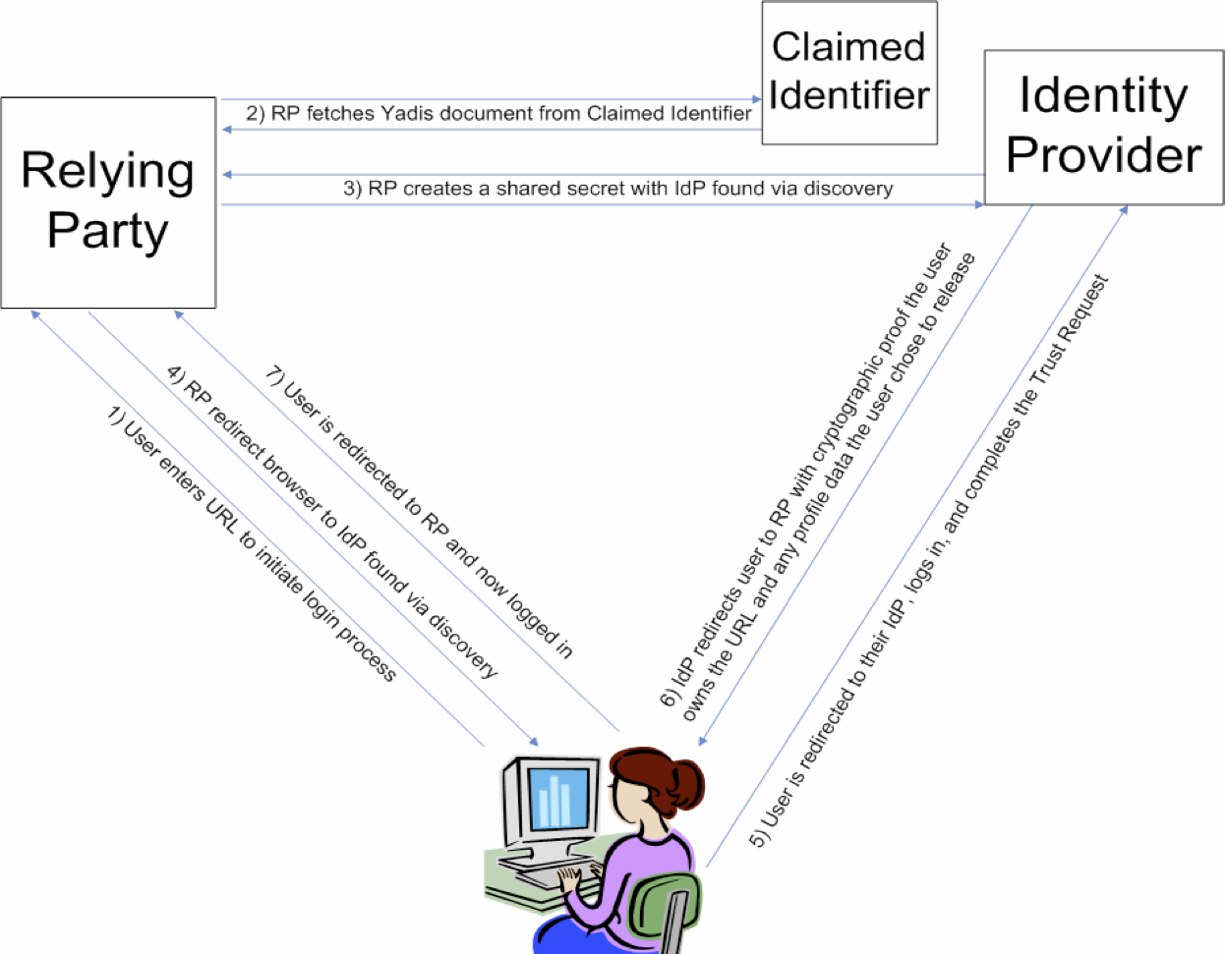
\includegraphics[width=0.9\textwidth]{images/openid_flow_recordon06.jpg}
        \caption{Basic OpenID Authentication Flow \cite{openid_2.0_platform_2009}}
        \label{fig:basic_openid_flow}
      \end{figure}


\subsection{OpenID:n heikkouksia}

OpenID-protokollasta on dokumentoitu lukuisia heikkouksia \cite{blackhat_openid_security_story, cameron_infocard_07, three_types_of_openid_ids_10}, joista merkittävimmät on selitetty jäljempänä olevassa listauksessa.

\begin{description}

  \item[1. Calastelu (\emph{phishing})] \hfill \\
    Pahantahtoinen sivu voi kysyä OpenID-tunnusta ja ohjata käyttäjän autenttista identiteetintarjoajaa matkivaan palveluun. Jos käyttäjä autentikoituu huijaussivulle salasanalla, käyttäjän OpenID-identiteetti päätyy vääriin käsiin. Korttiperustaisen autentikoinnin käyttäminen estäisi tämän haavoittuvuuden \cite{cameron_infocard_07}. Identiteetintarjoajista Yahoo! tarjoaa lisäsuojaa eräänlaisella ''vesileimalla'' \cite{yahoo_phishing_seal}.

   \item[2. Keskitetty riski] \hfill \\
      Jos OpenID-identiteetti päätyy vääriin käsiin, jokainen siihen kytketty palvelu on myös väärissä käsissä. 
      Riskinä tämä vertautuu sähköpostitunnuksen salasanan kadottamiseen, koska yleensä erinäisten palvelujen 
      salasananpalautustoiminnot lähettävät tarkisteen käyttäjälle suojaamattomassa sähköpostissa.
   
   \item[3. Luottamus identiteetintarjoajaan] \hfill \\
      Kaikki sisäänkirjautumistiedot ovat palveluntarjoajalla, jos tunnistautuminen kohdepalveluun tehdään
      osoiteperusteisella identiteetillä. Tällöin kohdepalvelu edellyttää käyttäjältä
      ainoastaan identiteetintarjoajaan kytketyn käyttäjätunnuksen haltijuuden todentamista.
      Asiakassertifikaatin (\emph{client certificate}) tai korttiperusteisen identiteetin käyttäminen
      lisätunnisteena ei tuo lisäturvaa, koska sellaisen vaatiminen on ainoastaan
      identiteetintarjoajan ja käyttäjän välinen asia.
      
   \item[4. Luottamus pysyvyyteen] \hfill \\
      Jos identiteetintarjoaja lopettaa toimintansa pysyvästi, siihen kytketyt tunnisteet eivät ole enää 
      käytettävissä. Ongelmaa on mahdollista kiertää kytkemällä palveluihin useampi eri OpenID-identiteetti. 
      Tämä kuitenkin lisää monimutkaisuutta, kun käytettäviä palveluja ja identiteettejä on useita.

  \item[5. Tunnisteiden kierrättäminen] \hfill \\
    Identiteetintarjoaja ei saisi antaa kerran käytössä ollutta OpenID-osoitetta enää ikinä kenellekään.
    Jos käyttäjä poistaa OpenID-identiteettinsä identiteetintarjoajalta, käyttäjän täytyy poistaa sitä vastava 
    OpenID-osoite
    myös \emph{kaikista} palveluista, joissa sitä on käytetty.
   
  \item[5. Luottamus DNS-protokollaan] \hfill \\
    OpenID-protokollan mukaisesti kohdepalvelu ei tunne käyttäjän identiteetintarjoajaa etukäteen.    
    Jos DNS-kyselyihin ei saada autenttista vastausta, palvelu voi johtaa käyttäjän oikeaksi naamioituneelle,
    huijaukseen osallistuvalle identiteetintarjoajalle. Vaatimalla osoiteperusteinen käyttäjätunnus
    etuliitteellä \emph{https://} ja DNSSec-laajennoksen yleistyminen lieventävät riskiä.

   \item[6. Epätasa-arvoiset identiteetintarjoajat] \hfill \\
      Monet suuret palvelut, kuten Google, Facebook, Microsoft MSN, Yahoo, tarjoavat OpenID-tunnisteen, jota
      voi käyttää sisäänkirjautumiseksi muihin palveluihin. Yksikään näistä ei kuitenkaan hyväksy
      sisäänkirjautumista omaan palveluunsa muulla kuin itsensä myöntämällä OpenID-käyttäjätunnuksella.
      
\end{description}

   
\subsection{Sama OpenID-identiteetti ei käy kaikkiin palveluihin}

OpenID-standardi tarjoaa laajalle levinneen autentikointiprotokollan, jolle on tarjolla laaja ja kypsä kirjastotuki \cite{openid_libraries}. Selvin OpenID:n hyöty on saman käyttäjätunnuksen käyttäminen monessa palvelussa ilman salasanan jakamista näiden palvelujen kesken. Koska käyttäjän itsensä tarvitsee autentikoitua ainoastaan identiteetintarjoajalle -- yhteen palveluun -- voidaan tämä nimenomainen sisäänkirjautuminen tehdä mahdollisimman turvalliseksi \cite{blackhat_openid_security_story}. Salasanan sijaan tai sen lisäksi käyttäjältä voidaan edellyttää korttiperusteista identiteettiä \cite{cameron_infocard_07} tai asiakassertifikaattia \cite{henry_story_foaf_ssl}. OpenID:n saavutuksena on, että vaihtoehtoinen tai rinnakkainen autentikoitumismenetelmä riittää toteuttaa ainoastaan yhteen palveluun eli identiteetintarjoajaan.

Yleinen tapa OpenID:n soveltamiselle on hyväksyä ainoastaan ennalta määritetty joukko (\emph{whitelist})
OpenID-identiteetintarjoajia \cite{openid_seven_sites_mailinglist, openid_tech_or_movement}. 
Jos palvelu ei hyväksy vapaavalintaista OpenID-identiteetintarjoajaa, hyväksyttyjä tarjoajia ovat usein ainoastaan suuret palveluntarjoajat (Google, Facebook, Microsoft, Yahoo), jotka hyväksyvät ainoastaan itsensä
myöntämän OpenID-tunnisteen. Tämän seurauksena käyttäjällä on väistämättä monta eri OpenID-identiteettiä,
jolloin käyttäjällä on myös tarve monelle eri salasanalle.

OpenID vähentää salasanojen kokonaismäärää, mutta se ei auta pääsemään eroon kaikista palvelukohtaisista
salasanoista. Keskimääräisellä käyttäjällä on tunnus 25:ssä eri palvelussa \cite{study_of_passwords_07}.
Kuitenkin esimerkiksi kirjoittajalla on tällä hetkellä käyttäjätunnus noin 60:ssa eri web-palvelussa. Vaikka
OpenID olisi tuettu 50~\%:ssa näissä palveluissa, palvelukohtaisia salasanoja olisi edelleen kolmekymmentä.
Googlen listauksessa webin suosituimmista palveluista \cite{google_top1000_sites} yksikään suosituimmista 50:sta
palvelusta ei hyväksy kuin itsensä tai taustayrityksensä myöntämän käyttäjätunnuksen.



\section{Salasanat ovat vallitseva käytäntö}
  \label{sec:passwords_de_facto}

Salasana on palvelun toimittajan kannalta kustannustehokas autentikoitumismenetelmä, ja siksi salasanat ovat olleet vallitsevin tunnistamistapa vuosikymmenten ajan \cite{pw_auth_system_perspective_08}. Kuten kappaleessa~\ref{sec:passwords} esiteltiin, käyttäjillä on keskimäärin 6,5 eri salasanaa, joista jokainen on jaettu keskimäärin 3,9 eri palvelun kesken \cite{study_of_passwords_07}. Lisäksi salasanojen jakaminen, yksinkertaisuus, unohtaminen, vaihtumattomuus ja arvattavuus on hyvin yleistä \cite{password_management_strategies_06, pw_auth_system_perspective_08, passpet_06}.

Helposti muistettavat salasanat, kuten luonnollisen kielen sanat, niiden johdannaiset tai nimet, ovat haavoittuvaisia \emph{sanakirjahyökkäykselle}, jossa hyökkääjä yrittää arvata salasanoja käyttäen ennalta valitun sanakirjan sanoja sekä niiden muunnoksia \cite{users_are_not_the_enemy_99, passpet_06}. Salasanan säännöllinen vaihtaminen pienentää todennäköisyyttä väkisinarvaamisen onnistumiseen, jos jonkin käytetyn palvelun salasanat ovat päätyneet vääriin käsiin. Saman salasanan tai sen johdannaisten käyttäminen monessa eri palvelussa vaarantaa käyttäjätunnuksen turvallisuuden, mutta eri salasanan muistaminen moneen palveluun ja salasanan vaihtaminen usein kuitenkin on epätoivoinen taakka ihmisille \cite{password_management_strategies_06, passpet_06, pw_auth_system_perspective_08, users_are_not_the_enemy_99}.

Ihmiset unohtavat salasanansa säännöllisesti \cite{ponemon_pw_survey_06, password_management_strategies_06}. Florêncion ja Herleyn 500.000 käyttäjän tutkimuksessa \cite{study_of_passwords_07} esimerkiksi Yahoon salasananvaihtotoimintoa käytettiin 15~\% yhtä usein kuin sisäänkirjautumista. Microsoft UK:n salasanaselvityksen mukaan neljäsosa (27~\%) briteistä unohtavat salasanansa säännöllisesti \cite{microsoft_pw_survey_04}. Lähes puolet 46~\% käyttäjistä kertoivat helpon muistettavuuden ja 71~\% salasanan vahvuuden olevan yksi tärkeimmistä kriteereistä salasanan valinnassa \cite{symantec_pw_survey_10}. Kuitenkin salasana kirjoitetaan usein paperilapulle, joka sijoitetaan näppäimistön alle \cite{pw_auth_system_perspective_08}.

 % - ihmiset käyttävät samaa salasanaa pitkään (paha yhdistettynä muihin ongelmiin)
 % - huono salasana jaetaan useammin kuin hyvä \cite{study_of_passwords_07}
 % - phishing: datan \cite{study_of_passwords_07} perusteella 0,4 \% internetin käyttäjistä falls victim to a phishing attack a year
 % - twitter adminin salasana murrettu sanakirja hyökkäyksellä, seurauksena lukuisia suosittuja käyttäjäprofiileja kaapattiin: http://www.codinghorror.com/blog/2009/01/dictionary-attacks-101.html
%     - admin käytti heikkoa salasanaa JA palvelu salli rajoittamattoman määrän yrityksiä

\subsection{Vaatimukset pilviyhteensopivalle autentikoinnille}

  \begin{quote}
      ''The fool saith, 'Put not all thy eggs in one basket' ... 
      but the wise man saith, 'Put all your eggs in one basket, and watch that basket!' ''
      \\--- Mark Twain \cite{twain_eggs_1894}
  \end {quote}

Mikään yksittäinen autentikointimenetelmä ei sovi kaikkiin tilanteisiin \cite{will_we_ever_escape_passwords_05}.
Salasanoja tarvitaan niin kauan kuin salasanan sijasta ei ole käytännössä mahdollista vaatia turvallisempaa autentikointitapaa, kuten sertifikaatit, avaimet ja ulkoiset laitteet -- jokaisessa palvelussa.
Salasanat eivät kuitenkaan itsessään ole tietoturvaketjun heikoin lenkki. Salasanat pystyvät vastaamaan tiukkoihinkin turvallisuusvaatimuksiin, kunhan niitä käytetään täsmällisesti \cite{will_we_ever_escape_passwords_05}.

Kappaleessa~\ref{sec:passwords_de_facto} todetun perusteella yhtä salasanaa ei pitäisi käyttää kuin yhdessä palvelussa. Lisäksi jokaisen salasanan tulisi olla vahva. Koska käyttäjän ei ole mahdollista muistaa monen erilaisen vahvan salasanan \emph{lisäksi} sitä, mihin palveluun mikäkin salasana käy, tarvitaan salasanojen hallintaa. On asiantuntijoita, joiden mielestä vahvan salasanan (tai sen osan) kirjoittaminen lompakossa säilytettävälle paperilapulle on turvallista \cite{fsecure_passwords_on_postit_09, microsoft_guru_write_your_password_05, schneier_changing_passwords_10, schneier_choosing_passwords_07, schneier_write_down_your_password_05}, kun samaan yhteyteen ei kirjoiteta käyttäjätunnusta tai palvelun nimeä. Salasanojen lukumäärän kasvaessa käy kuitenkin vaikeaksi muistaa, mihin palveluun mikäkin salasanoista sopii \cite{study_of_passwords_07}. 

Salasanojen turvallisuus on suunniteltava käyttäjälähtöisesti, tai muuten käyttäjä pyrkii kiertämään rajoitukset itse. Adams \emph{et al.} havaitsivat \cite{users_are_not_the_enemy_99}, että käyttäjät valitsevat vähemmän turvallisia salasanoja, kun palvelu vaatii salasanan vaihtamista säännöllisesti. Syynä on luonnollisesti se, että uusi salasana tuottaa uutta muistettavaa. Tutkimuksessa käyttäjät eivät ymmärtäneet tietoturvasäännöstön tarkoitusta, minkä vuoksi käyttäjät kokivat rajoitukset pakottamisena. Seuraus oli, että lukuisat tutkimuksen käyttäjistä päätyivät kiertämään turvallisuussääntöjä.

% Salasanan vanheneminen:
% ''The downside of changing passwords is that it makes them harder to remember. And if you force people to change their passwords regularly, they're more likely to choose easy-to-remember -- and easy-to-guess -- passwords than they are if they can use the same passwords for many years. So any password-changing policy needs to be chosen with that consideration in mind.''
% http://www.schneier.com/blog/archives/2010/11/changing_passwo.html
% 
% Jos käyttäjää vaaditaan vaihtamaan liian salasana usein, käyttäjän seuraavat salasanat ovat johdannaisia, jotka on mahdollista arvata jos tiedetään ensimmäinen salasana.
% \cite{password_expiration_10}
% 
% ''Password expiration does not offer any benefit when a nattacker wants to do all of the damage that he's going to do right now. It does offer a benefit when the attacker intends to continue accessing a system for an extended period of time.''
% https://lopsa.org/node/295
% -- S. Alexander, Jr. In defense of password expiration. Post to LOPSA blog, April 2006.

parapara \cite{generating_and_remembering_pws_04, password_management_strategies_06}


\subsection{Tavoitteet salasanojen turvallisuudelle}

Ilman hallintaohjelmista näitä sääntöjä tulee rikottua.
\cite{why_phishing_works_06}

\begin{description}

  \item[1. Salasana generoidaan vahvaksi.] \hfill \\
    Salasana voidaan generoidaan ilman käyttäjän vuorovaikutusta. 
    Jos käyttäjän annetaan kehittää salasana itse, täytyy ohjelman arvioida salasanan vahvuus.
    Käyttäjät arvioivat helposti salasanan vahvuuden väärin \cite{password_management_strategies_06}. 
    Esimerkiksi salasana ''Sn00py'' voi olla kryptografisesti vahvempi kuin ''123456'', mutta
    sanakirjahyökkäyksessä eroa ei välttämättä ole. Myös profiilitiedot käyttäjästä nopeuttavat murtumista, jos 
    esimerkiksi tiedetään ''Snoopyn'' olevan käyttäjän suosikkisarjakuvahahmo ja salasana on ''Sn00py''.
     
  \item[2. Yhtä salasanaa käytetään vain yhdessä palvelussa.] \hfill \\
   Tavoitteena on estää tilanne, jossa yhden salasanan joutuminen vääriin käsiin vaarantaisi käyttäjän tiedot
   muissa palveluissa. Jos jokaisessa palvelussa on eri salasana, tietomurron aiheuttama vahinko rajoittuu
   murron kohteena olevaan palveluun.

  
  \item[3. Salasanat eivät ole johdannaisia toisistansa.] \hfill \\
    Yhden tai useamman salasanan ei perusteella ei saa voida arvata tai tuottaa muita salasanoja. Jos käyttäjän
    salasana esimerkiksi Facebookiin on ''faceYhfmn2\#3'' ja Gmailiin ''gmaYhfmn2\#3'', helpottuu Yahoo-tunnuksen
    salasanan murtaminen merkittävästi. Hyökkääjän riittää kokeilla kaikki palvelun nimestä johdettavat
    kombinaatiot ja liittää niihin muista salasanoista tunnetut yhteiset osat.
  
  \item[4. Käyttäjän ei tarvitse tietää palvelussa käyttämäänsä salasanaa.] \hfill \\
    Tavoitteena on vähentää käyttäjän muistin kuormitusta.
    Toisin sanoen tavoitteena on siirtää vastuu salasanojen hallinnasta
    mahdollisimman suurelta osin on salasanojen hallintaohjelmiston tehtäväksi.
    Koska käyttäjä ei tunne salasanaansa, salasanaa ei ole mahdollista huijata käyttäjältä.
    Salasanan huijaaminen hallintaohjelmistolta, jos käyttäjä antaa siihen itse luvan, on tosin edelleen
    mahdollista.
  
  \item[5. Käyttäjän tarvitsee muistaa vain yksi vahva salasana.] \hfill \\
    salainen lause  (\emph{passphrase})

\end{description}


\subsection{Tavoitteet salasanojen hallinnalle}

\begin{description}

  \item[1. Käyttäjä pääsee käsiksi salasanoihin miltä tahansa työasemalta.] \hfill \\
    Loerem ipspspssum dolem amet sit ja niin edelleen
    
  \item[2. Salasanat sisältävä kokoelma talletetaan verkossa olevaan palveluun.] \hfill \\
      Loerem ipspspssum dolem amet sit ja niin edelleen
      
  \item[3. Salasanakokoelmaa säilytetään verkossa kryptatussa muodossa.] \hfill \\
      Loerem ipspspssum dolem amet sit ja niin edelleen
      
  \item[4. Kryptauksen salausavainta ei koskaan välitetä verkon yli.] \hfill \\
      Loerem ipspspssum dolem amet sit ja niin edelleen

\end{description}

Kryptauksessa käytetty salausavain johdetaan käyttäjän salaisesta lauseesta.
- tai käytetään salausavaimena käyttäjän salasanaa
- valinta: pitääkö salausavain muistaa? kirjoitetaanko se lompakkoon?

Salasanojen purkaminen suoritetaan web-selaimessa selainlaajennoksen avulla.




\subsection{Katsaus olemassaoleviin toteutuksiin}
\subsection{}
\subsection{Rajoitteet}
 - Jokaiselle selaimelle oma plugin
 - Spyware ja MITM. 
 - DNS: Oletetaan että DNS palauttaa oikean IP osoitteen
 - Fokuksen varastaminen
 
% \section{Related Work}
%   Kamouflage: loss-resistant password management
%   http://portal.acm.org/citation.cfm?id=1888881.1888904&coll=DL&dl=GUIDE&CFID=2580387&CFTOKEN=49759375
%   
%   Secure passwords through enhanced hashing
%   http://portal.acm.org/citation.cfm?id=1855698.1855705&coll=DL&dl=GUIDE&CFID=2580387&CFTOKEN=49759375
%   
%   Passpet: convenient password management and phishing protection
%   http://portal.acm.org/citation.cfm?id=1143120.1143126&coll=DL&dl=GUIDE&CFID=2580387&CFTOKEN=49759375
  
  
\section{Jatkotutkimuksia}

   \subsection{WebID}
      \cite{webid_home}
      % http://esw.w3.org/WebID#How_does_the_WebID_Protocol_compare_with_OpenID.3F

   \subsection{Firefox Sync, Chromium Sync}
     % Chromium sync 
     %  https://groups.google.com/group/chromium-dev/browse_frm/thread/bdacc1bdf3c5cb6a?hl=en&pli=1
     %  Password sync coming probably soon, tavoite 6.0 beta
     %    http://www.readwriteweb.com/archives/google_chrome_gets_extension_sync.php
     %  "The team is working on it"
     %    https://www.google.com/support/forum/p/Chrome/thread?tid=6d4d3953859d6a9b&hl=en
     %  Chrome Cloud synchronization, google
     %    http://arstechnica.com/open-source/news/2009/08/google-reveals-plans-for-chrome-cloud-synchronization.ars
     %  The protocol _is_ open.  Protobufs are open source and the sync spec built on them is also open source.
     %   https://groups.google.com/group/chromium-dev/browse_thread/thread/bdacc1bdf3c5cb6a
     

\section{Yhteenveto}
% http://www.codinghorror.com/blog/2008/05/openid-does-the-world-really-need-yet-another-username-and-password.html
% I realize that OpenID is far from an ideal solution. But right now, the one-login-per-website problem is so bad that I am willing to accept these tradeoffs for a partial worse is better solution. There's absolutely no way I'd put my banking credentials behind an OpenID. But there are also dozens of sites that I don't need anything remotely approaching banking-grade security for, and I use these sites far more often than my bank. The collective pain of remembering all these logins -- and the way my email inbox becomes a de-facto collecting point and security gateway for all of them -- is substantial. 
%        If we can't make OpenID work, at least for run of the mill, low-value credentials that litter the web in increasing numbers -- what hope do we have of ever fixing the login explosion problem? 

\bibliographystyle{tktl}
\bibliography{lahteet}

\lastpage

\end{document}